\documentclass{scrartcl}

\usepackage[usenames,dvipsnames,svgnames,table]{xcolor}
\usepackage{textcomp}
\usepackage{amssymb}
\usepackage{datetime}
\usepackage{graphicx}
\usepackage{gensymb}
\usepackage{wrapfig}
\usepackage{geometry}
\usepackage{caption}
\geometry{textwidth = 17cm,textheight = 24cm}

\begin{document}

%-------------------- begin header -------------------%
\centerline{\LARGE Process sheet for \textbf{vt01}}
\vspace{0.5em}
\centerline{\Large Physics and Hardware for Intelligence project}
\vspace{0.5em}
\centerline{\large Physical Measurement Laboratory, NIST Boulder}
\vspace{0.5em}
\centerline{Dated \today}
%-------------------- end header ---------------------%

\begin{figure}[!h]
\centering
\setlength{\fboxsep}{0pt}%
\setlength{\fboxrule}{0pt}%
\fbox{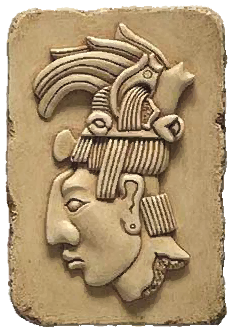
\includegraphics[width=3cm]{votan_white.png}}
%\caption*{Votan, the Mayan god of optical to electrical transduction.}
\end{figure}

%-------------------- begin summary ------------------%
%\vspace{1em}
\noindent \underline{Process overview:} Fabrication flow for the Nb/Si/Nb, externally shunted JJ process. This process includes a ground plane, JJ tri-layer, upper Nb wiring layer, and PdAu resistors.

The process starts with a thermally oxidized Si wafer with 160\,nm SiO$_2$. 

The entire wafer is clad with oxide, and openings are etched to the bond pads (\textbf{v4}). A Nb ground plane is deposited, and alignment marks are etched in this layer. Features are then etched in the ground plane (\textbf{m0}).

\vspace{2em}\noindent Insert screen shot of die and image distribution from stepper:

%\begin{figure} %[!b]
%\centering
%\includegraphics[width=17.2cm]{olmc_flowImages_17-fullWithCircuit.png}
%\caption*{Electrial-to-optical-to-electrical-to-optical-to-electrical transduction chain circuit diagram around which this fab process is designed.}
%\end{figure}
%-------------------- end summary -------------------%

%-------------------- begin steps -------------------%
\newpage
\noindent \underline{Step 1:} Etched alignment marks for ebeam and stepper (global ebeam, local ebeam, and ASML)
%\begin{figure}[!b]
%\centering
%\includegraphics[width=0.75\textwidth]{olmc_flowImages_01.png}
%\caption*{Step 1: SOI wafer with device layer exposed.}
%\end{figure}

\vspace{0.5em}
GDS layer(s): none/shared marks reticle
%\begin{itemize} 
%\input{../_fabricationSteps/etch_etchedEbeamMarks_soi_01}
%\end{itemize}
%\vspace{1em}
%\noindent Additional notes: \input{../_fabricationSteps/notes_ebeamMarks_01} \input{../_fabricationSteps/notes_ebeamMarks_etched_01}
%-------------------- step break --------------------%
\newpage
\noindent \underline{Step 2:} Clean wafer and deposit protective SiO$_2$ for implants and anneal
%\begin{figure}[!b]
%\centering
%\includegraphics[width=0.75\textwidth]{olmc_flowImages_02.png}
%\caption*{Step 2: SOI wafer with protective oxide.}
%\end{figure}

\vspace{0.5em}
GDS layer(s): none/full wafer
%\begin{itemize}
%\input{../_fabricationSteps/clean_nanostrip_01}
%\input{../_fabricationSteps/dep_SiO2_protective_01}
%\end{itemize}
%\vspace{1em}
%\noindent Additional notes: \input{../_fabricationSteps/notes_dep_opto-SiO2_01}
%\vspace{1em}
\noindent Insert endpoint signal and logbook screenshots here.
%-------------------- step break --------------------%
\newpage
\noindent \underline{Step 26:} Dice wafer
\vspace{0.5em} \newline
GDS layer(s): none / full wafer
%\begin{itemize}
%\input{../_fabricationSteps/misc_dice_01}
%\end{itemize}
\vspace{1em}
\noindent Additional notes: Insert microscope screen shots if desired. 
%-------------------- end steps ---------------------%

%\begin{figure}[!b]
%\centering
%\includegraphics[width=17.2cm]{olmc_flowImages_17-fullWithCircuit.png}
%\caption*{Circuit, side view, and top view after fabrication is complete.}
%\end{figure}

\end{document}